% Pairwise Independence of Representation, Classification, and Composition
% in Finite Extensional Magmas
% arXiv preprint
\documentclass[sigconf,screen]{acmart}

% Lean code listings
\usepackage{listings}
\lstset{
  basicstyle=\ttfamily\small,
  columns=flexible,
  breaklines=true,
  frame=none,
  xleftmargin=1em,
}

% TikZ for independence diagram
\usepackage{tikz}
\usetikzlibrary{arrows.meta,positioning,decorations.markings}

% Shortcuts
\newcommand{\dotop}{\cdot}
\newcommand{\FRM}{\textsf{FRM}}
\newcommand{\ICP}{\textsf{ICP}}
\newcommand{\Fin}{\mathrm{Fin}}
\newcommand{\core}{\mathrm{core}}
\newcommand{\Nat}{\mathbb{N}}

% Additional theorem environments (ACM provides theorem, lemma, corollary, proposition, definition)
\newtheorem{observation}{Observation}
\theoremstyle{remark}
\newtheorem{remark}{Remark}

\begin{document}

\title{Pairwise Independence of Representation, Classification, and Composition in Finite Extensional Magmas}
\thanks{Preprint version.}

\author{Stefano Palmieri}
\affiliation{
  \institution{Independent Researcher}
  \city{Austin}
  \state{Texas}
  \country{USA}
}

\begin{CCSXML}
<ccs2012>
<concept>
<concept_id>10003752.10003790.10003795</concept_id>
<concept_desc>Theory of computation~Algebraic language theory</concept_desc>
<concept_significance>500</concept_significance>
</concept>
<concept>
<concept_id>10003752.10003790.10002990</concept_id>
<concept_desc>Theory of computation~Logic and verification</concept_desc>
<concept_significance>500</concept_significance>
</concept>
</ccs2012>
\end{CCSXML}

\ccsdesc[500]{Theory of computation~Algebraic language theory}
\ccsdesc[500]{Theory of computation~Logic and verification}

\keywords{finite extensional magma, pairwise independence, self-simulation, classifier dichotomy, Lean~4, machine-checked proofs}

\begin{abstract}
Partial combinatory algebras (PCAs), total combinatory algebras (TCAs), and Turing categories provide the algebraic and categorical foundations of computability. All three study what can be computed or how computability composes. These frameworks analyze which functions are representable and how algebras relate to each other, but not the partition of individual elements into behavioral types by their row structure in the operation table, or the algebraic constraints that such partitions impose. In the setting of finite extensional 2-pointed magmas --- total binary operations on finite sets with two distinguished absorbers and extensionality --- we identify three algebraic properties associated with self-simulation: self-representation~(R), the classifier dichotomy~(D), and the Internal Composition Property~(H). We prove these three properties are pairwise independent: six Lean-verified finite counterexamples (sizes $5$--$10$) establish all six non-implications. The minimum self-simulating coexistence witness has $N\!=\!5$ (Lean-verified), which is optimal: ICP requires 3 pairwise distinct core elements, so $N \geq 5$. We also prove that self-simulation forces discrimination (the partial application map must be injective), that associativity is incompatible with the classifier structure (ruling out semigroups, monoids, groups, and rings), and that the three-category decomposition induced by D is an isomorphism invariant. A classical result shows that nontrivial combinatory algebras with S and K must be infinite; our finite magmas avoid this obstruction by using left-absorbers instead of a K combinator, enabling an algebraic analysis of self-simulation that the infinite PCA/TCA setting obscures. All results are formalized in Lean~4 with zero \texttt{sorry}.
\end{abstract}

\maketitle

% ══════════════════════════════════════════════════════════════
\section{Introduction}
\label{sec:introduction}
% ══════════════════════════════════════════════════════════════

Partial combinatory algebras (PCAs)~\cite{vanoosten08,longley15}, total combinatory algebras (TCAs)~\cite{bethke88}, and Turing categories~\cite{cockett08} provide the algebraic and categorical foundations of computability. PCA theory studies what is computable from a given set of realizers, including detailed analysis of morphisms, quotients, and totalizability~\cite{bethke96}. TCA theory studies when application can be made total. Turing category theory axiomatizes the categorical structure of computability. These frameworks study which functions are representable and how algebras relate to each other, but not the \emph{partition} of individual elements into behavioral types by their row structure in the operation table --- the question of whether classifiers and non-classifiers form disjoint classes, and what algebraic constraints that partition imposes.

There is a structural reason for this omission. Nontrivial combinatory algebras with $\mathbf{s}$ and $\mathbf{k}$ are necessarily infinite: the $\mathbf{k}$ combinator provides a non-surjective injection on the ground set (Theorem~\ref{thm:k-infinity}). Finite algebras fall outside the PCA/TCA framework entirely. We show that finite extensional magmas --- total binary operations on finite sets --- support a rich algebraic analysis of self-simulation that the infinite setting obscures.

We work in the setting of finite extensional 2-pointed magmas (a finite set with a binary operation, exactly two left-absorbers, and extensionality; the framework follows universal algebra~\cite{burris81}). We study three algebraic properties that arise as components of self-simulation --- computing one's own operation table from within --- but are independently formalizable: self-representation~(R), the existence of a section-retraction pair on the non-absorber elements (the \emph{core}); the classifier dichotomy~(D), a clean partition of core elements into those whose action on core lands entirely in the absorbers and those whose action avoids them entirely; and the Internal Composition Property~(H), the existence of a non-trivial factorization in the left-regular representation restricted to core. Each property has an independent algebraic motivation (Section~\ref{sec:discussion}), and self-simulation provides a unifying computational context in which all three co-occur (Section~\ref{sec:selfsim}). Our main result is that R, D, and H are pairwise independent: no one implies any other.

Six Lean-verified finite counterexamples of sizes $N\!=\!5, 6, 8,$ and $10$ establish all six non-implications; coexistence witnesses at $N\!=\!5$ and $N\!=\!6$ show all three can hold simultaneously, and both self-simulate. The $N\!=\!5$ bound is optimal: ICP requires 3 pairwise distinct core elements, forcing $|S| \geq 5$. Each counterexample is a concrete Cayley table found by SAT search and independently verified in Lean~4~\cite{moura21}, zero \texttt{sorry}.

The three properties arise naturally in the study of reflective computation. Smith's 3-Lisp~\cite{smith84}, Friedman and Wand's reification~\cite{friedman84}, Amin and Rompf's collapsed towers~\cite{amin18}, and Brown and Palsberg's typed self-interpreters~\cite{brown16} all combine representation, classification, and composition without separating them. In the finite algebraic setting, we show that this bundling is not structurally forced; whether the independence extends to $\lambda$-calculus or typed settings is an open question (Section~\ref{sec:discussion}).

Beyond independence, we prove several additional structural results. Self-simulation forces discrimination: any self-simulating algebra must produce $n$ distinct intermediate terms for $n$ elements (Theorem~\ref{thm:injectivity}). Universal obstructions rule out the classical algebraic hierarchy: no extensional 2-pointed magma carrying both a classifier and a retraction pair has a right identity or is associative (Theorem~\ref{thm:no-assoc}). The three-category decomposition induced by~D is an algebraic invariant (Theorem~\ref{thm:functoriality}), and the ICP is equivalent to the standard Compose+Inert axioms (Theorem~\ref{thm:icp-equiv}).

The setting of finite extensional 2-pointed magmas is not an arbitrary choice but is forced by known obstructions. The K-infinity theorem (Theorem~\ref{thm:k-infinity}) rules out finite combinatory algebras: any nontrivial algebra with a $\mathbf{k}$ combinator must be infinite. The no-associativity theorem (Theorem~\ref{thm:no-assoc}) rules out semigroups, monoids, groups, and rings: associativity collapses any classifier to an absorber. Extensionality is required for the discrimination theorem (Theorem~\ref{thm:injectivity}): the final step derives element equality from identical rows. Two absorbers are required for binary classification (the classifier must distinguish at least two outcomes). Such magmas are the minimal remaining setting after these obstructions.

\paragraph{Contributions.}
\begin{enumerate}
  \item An independence theorem: R, D, and H are pairwise independent, with Lean-verified counterexamples in all six directions at $N\!=\!5$ through $N\!=\!10$ (Section~\ref{sec:independence}), and self-simulating coexistence witnesses at $N\!=\!5$ and $N\!=\!6$ (Sections~\ref{sec:selfsim} and~\ref{sec:bound}).
  \item An optimal bound: $N\!=\!5$ is the minimum carrier size for R+D+H coexistence, and both the $N\!=\!5$ and $N\!=\!6$ witnesses self-simulate (Lean-verified). ICP is impossible at $N\!=\!4$ by pigeonhole (Theorem~\ref{thm:no-icp-4}). Self-simulation also forces the partial application map to be injective (Theorem~\ref{thm:injectivity}).
  \item Universal algebraic obstructions: no extensional 2-pointed magma carrying both a classifier and a retraction pair has a right identity or is associative, ruling out semigroups, monoids, groups, and rings (Section~\ref{sec:universal}).
  \item Decomposition invariance: the three-category partition is preserved by isomorphisms (Section~\ref{sec:invariance}).
  \item A characterization of H confirming the ICP is not ad hoc: it is logically equivalent to Compose+Inert under variable renaming, with necessity of the non-degeneracy conditions demonstrated by Lean-verified witnesses (Section~\ref{sec:icp}).
\end{enumerate}

% ══════════════════════════════════════════════════════════════
\section{Definitions}
\label{sec:definitions}
% ══════════════════════════════════════════════════════════════

Throughout, $(S, \dotop)$ is a finite magma on $\Fin(n) = \{0, 1, \ldots, n-1\}$ with binary operation $\dotop : \Fin(n) \times \Fin(n) \to \Fin(n)$.

\begin{definition}[Extensional 2-Pointed Magma]
\label{def:epm}
An \emph{extensional 2-pointed magma} is a tuple $(S, \dotop, z_1, z_2)$ where:
\begin{enumerate}
  \item $z_1, z_2 \in S$ are distinct \emph{left-absorbers}: $z_i \dotop x = z_i$ for all $x$.
  \item No other element is a left-absorber.
  \item \emph{Extensionality}: if $a \dotop x = b \dotop x$ for all $x$, then $a = b$.
\end{enumerate}
We write $\core(S) := S \setminus \{z_1, z_2\}$ for the non-absorber elements.
\end{definition}

\begin{definition}[Faithful Retract Magma]
\label{def:frm}
A \emph{Faithful Retract Magma} $(\FRM)$ extends an extensional 2-pointed magma with a \emph{retraction pair} $s, r \in \core(S)$ satisfying $r \dotop (s \dotop x) = x$ for all $x \in \core(S)$, with $r \dotop z_1 = z_1$ (anchoring). The remaining absorber outputs of $s$ and $r$ are unconstrained.
\end{definition}

\begin{remark}[Retraction pair convention]
\label{rem:mutual}
Throughout this paper, the retraction pair $(s, r)$ satisfies mutual inverse on core: $r \dotop (s \dotop x) = x$ and $s \dotop (r \dotop x) = x$ for all $x \in \core(S)$. This matches the Lean formalization. Most theorems (9 of 11) require only the one-sided condition $r \dotop (s \dotop x) = x$; two results --- retraction pair placement (both $s, r \in N$; Theorem~\ref{thm:placement}) and the tight bound $|S| \geq 5$ when $s \neq r$ (Theorem~\ref{thm:card}) --- use the full mutual inverse. We adopt the stronger convention for uniformity and note the weaker hypotheses where relevant.
\end{remark}

The retraction pair provides encoding infrastructure: element $a$ can be represented as $s^k(z_1)$ for its index $k$, and $r$ peels one layer. Informally, this acts as a finite internal coding scheme, analogous in spirit to a G\"odel numbering.

\begin{definition}[Classifier Dichotomy]
\label{def:cd}
An extensional 2-pointed magma satisfies the \emph{classifier dichotomy} when:
\begin{enumerate}
  \item A \emph{classifier} $\tau \in \core(S)$ exists with $\tau \dotop x \in \{z_1, z_2\}$ for all $x$.
  \item For every $y \in \core(S)$, either
    \begin{itemize}
      \item $y \dotop x \in \{z_1, z_2\}$ for all $x \in \core(S)$ \quad ($y$ is a \emph{classifier}), or
      \item $y \dotop x \notin \{z_1, z_2\}$ for all $x \in \core(S)$ \quad ($y$ is a \emph{non-classifier}).
    \end{itemize}
  \item At least one non-classifier exists (excluding the degenerate case where the ``dichotomy'' has only one inhabited class).
\end{enumerate}
\end{definition}

The dichotomy creates a three-category decomposition $S = Z \sqcup C \sqcup N$ where $Z = \{z_1, z_2\}$ (absorbers), $C$ (classifiers), and $N$ (non-classifiers). No element can be partially classifying. We call elements in $\{z_1, z_2\}$ \emph{absorber-valued} (abbreviated \emph{boolean-valued} when the absorbers play the role of truth values).

\begin{definition}[Internal Composition Property]
\label{def:icp}
A magma $(S, \dotop, z_1, z_2)$ satisfies the \emph{Internal Composition Property} $(\ICP)$ when:
\[
\exists\, a, b, c \in \core(S),\ \text{pairwise distinct, such that:}
\]
\begin{enumerate}
  \item \emph{Core-preservation}: $b \dotop x \notin \{z_1, z_2\}$ for all $x \in \core(S)$.
  \item \emph{Factorization}: $a \dotop x = c \dotop (b \dotop x)$ for all $x \in \core(S)$.
  \item \emph{Non-triviality}: $|\{a \dotop x : x \in \core(S)\}| \geq 2$.
\end{enumerate}
\end{definition}

ICP says: the left-regular representation admits a non-trivial factorization on core. One core action factors through two others, one of them core-preserving --- a single fragment of internal composition. In Section~\ref{sec:icp} we prove that $\ICP$ is equivalent to the standard operational axioms Compose+Inert (Theorem~\ref{thm:icp-equiv}).

\begin{definition}[Capability R]
An extensional 2-pointed magma has capability $R$ (self-representation) if it admits a retraction pair. (We write R rather than S to avoid overloading with the carrier set~$S$.)
\end{definition}

\begin{definition}[Capability D]
An extensional 2-pointed magma has capability $D$ (self-description) if it satisfies the classifier dichotomy (Definition~\ref{def:cd}: existence of a classifier, the global dichotomy, and non-degeneracy).
\end{definition}

\begin{definition}[Capability H]
An extensional 2-pointed magma has capability $H$ (self-execution) if it satisfies the $\ICP$.
\end{definition}

All three capabilities are properties of the same base structure (Definition~\ref{def:epm}). None is defined as an extension of any other, making the independence theorem (Section~\ref{sec:independence}) a statement about six non-implications, all proved by Lean-verified counterexamples.

% ══════════════════════════════════════════════════════════════
\section{Universal Theorems}
\label{sec:universal}
% ══════════════════════════════════════════════════════════════

The following theorems are proved by pure algebraic reasoning (no \texttt{decide}) and formalized in \texttt{CatKripkeWallMinimal.lean} and \texttt{NoCommutativity.lean}. We state the hypotheses explicitly: some require only D, while others use both R and D.

\subsection{Theorems from D alone}

\begin{theorem}[Three-Category Decomposition]
\label{thm:three-cat}
In any extensional 2-pointed magma satisfying D, every element is a zero, a classifier, or a non-classifier. The classes are pairwise disjoint: in particular, $C \cap N = \emptyset$ (no element is partially classifying).
\end{theorem}

\begin{theorem}[Asymmetry]
\label{thm:asymmetry}
No extensional magma with two distinct left-absorbers is commutative.
\end{theorem}

\subsection{Theorems from R+D}

\begin{theorem}[Retraction Pair Placement]
\label{thm:placement}
In any extensional 2-pointed magma satisfying both R and D, any witness $r$ to R is a non-classifier: $r \in N$. (Under the stronger mutual-inverse condition in the Lean formalization, $s \in N$ also holds.)
\end{theorem}

\begin{theorem}[Cardinality Bounds]
\label{thm:card}
$|S| \geq 4$ for any extensional 2-pointed magma satisfying both R and D. (The bound $|S| \geq 4$ is nearly immediate from the definitions --- two absorbers, one classifier, one non-classifier --- but the Lean-verified proof confirms that no subtle interaction reduces it. The bound is tight: a 4-element witness with $s = r$ is exhibited in Appendix~\ref{app:tables}.) Under the stronger mutual-inverse condition with $s \neq r$, $|S| \geq 5$ (also tight); this is the nontrivial bound, as it shows the retraction pair consumes two distinct core slots.
\end{theorem}

\begin{theorem}[No Right Identity]
\label{thm:no-rid}
No extensional 2-pointed magma satisfying both R and D has a right identity element.
\end{theorem}

\begin{theorem}[No Associativity]
\label{thm:no-assoc}
No extensional 2-pointed magma carrying both a classifier and a retraction pair is associative. In particular, no extensional 2-pointed magma satisfying both R and D is a semigroup, monoid, group, or ring: the classifier dichotomy with a retraction pair is incompatible with the entire classical algebraic hierarchy.
\end{theorem}

\begin{proof}
Assume $(\tau \dotop a) \dotop b = \tau \dotop (a \dotop b)$ for all $a, b$. We derive a contradiction in four steps. The proof uses only extensionality, the existence of a classifier $\tau$, and a retraction pair $(s, r)$ --- neither the global dichotomy nor the non-classifier existence axiom is needed. Lean file: \texttt{CatKripkeWallMinimal.lean}.

\emph{Step 1: $\tau$ absorbs on the right.} For any $a, b$:
\[
\tau \dotop (a \dotop b)
= (\tau \dotop a) \dotop b
= z_i \dotop b
= z_i
= \tau \dotop a
\]
where the second equality uses $\tau \dotop a \in \{z_1, z_2\}$ (classifier), and the third uses left-absorption. So $\tau \dotop (a \dotop b) = \tau \dotop a$ for all $a, b$.

\emph{Step 2: $\tau$ is constant on core.} For any core $x$: the retraction pair gives $x = r \dotop (s \dotop x)$. Applying Step~1 with $a = r$, $b = s \dotop x$:
\[
\tau \dotop x = \tau \dotop (r \dotop (s \dotop x)) = \tau \dotop r.
\]
Set $v = \tau \dotop r \in \{z_1, z_2\}$. Then $\tau \dotop x = v$ for all core $x$.

\emph{Step 3: $\tau$ is constant on absorbers.} Since $\tau$ is a classifier, it hits both $z_1$ and $z_2$ --- otherwise, if $\tau \dotop x = z_1$ for all $x$, then $\tau$ and $z_1$ have identical rows, so $\tau = z_1$ by extensionality, contradicting $\tau \neq z_1$ (and symmetrically for $z_2$). Let $b_1, b_2$ witness $\tau \dotop b_1 = z_1$ and $\tau \dotop b_2 = z_2$. Applying Step~1 with $a = \tau$:
\[
\tau \dotop z_1 = \tau \dotop (\tau \dotop b_1) = \tau \dotop \tau = v,
\qquad
\tau \dotop z_2 = \tau \dotop (\tau \dotop b_2) = \tau \dotop \tau = v.
\]
The middle equalities use Step~1; $\tau \dotop \tau = v$ because $\tau$ is core (Step~2).

\emph{Step 4: Contradiction.} Steps 2 and 3 give $\tau \dotop x = v$ for all $x \in S$. Since $v \in \{z_1, z_2\}$, the classifier $\tau$ has the same row as absorber $v$. By extensionality, $\tau = v \in \{z_1, z_2\}$, contradicting $\tau \neq z_1, z_2$.
\end{proof}

\begin{remark}
The retraction pair is essential in Step~2: the identity $\tau \dotop x = \tau \dotop (r \dotop (s \dotop x)) = \tau \dotop r$ uses $r \dotop (s \dotop x) = x$ to show $\tau$ is constant on core. Without a retraction pair, the proof breaks, and the theorem does not extend to ``no extensional 2-pointed magma with a classifier is associative.''
\end{remark}

\subsection{The K-infinity obstruction}

The following classical result explains why the PCA/TCA framework cannot study finite algebras, and why our setting requires a different combinator basis.

\begin{theorem}[K-infinity]
\label{thm:k-infinity}
If $(A, \dotop, \mathbf{k}, \mathbf{s})$ is a combinatory algebra (total application satisfying $\mathbf{k} \dotop a \dotop b = a$ and the $\mathbf{s}$ equations) with $|A| \geq 2$, then $A$ is infinite.
\end{theorem}

\begin{proof}
The map $\varphi(x) = \mathbf{k} \dotop x$ is injective: $\mathbf{k} \dotop a = \mathbf{k} \dotop b$ implies $\mathbf{k} \dotop a \dotop c = \mathbf{k} \dotop b \dotop c$ for all $c$, hence $a = b$. We claim $\mathbf{k} \notin \mathrm{Im}(\varphi)$. Suppose $\mathbf{k} \dotop x = \mathbf{k}$ for some $x$. Then for all $y$, $\mathbf{k} \dotop x \dotop y = \mathbf{k} \dotop y$, so $x = \mathbf{k} \dotop y$ for all $y$. By injectivity, all $y$ are equal, contradicting $|A| \geq 2$. Thus $\varphi : A \to A$ is an injection missing $\mathbf{k}$, which is impossible for finite~$A$.
\end{proof}

\begin{remark}
The proof uses only the $\mathbf{k}$ equation ($\mathbf{k} \dotop a \dotop b = a$) and totality; $\mathbf{s}$ is irrelevant. Our extensional 2-pointed magmas avoid this obstruction: instead of a projector $\mathbf{k}$ with $\mathbf{k} \dotop a \dotop b = a$, they have left-absorbers $z$ with $z \dotop x = z$ (the dual pattern --- constant on columns, not rows) and a retraction pair $(s, r)$ with $r \dotop (s \dotop x) = x$ on core. Neither structure provides a non-surjective injection on the full ground set.
\end{remark}

% ══════════════════════════════════════════════════════════════
\section{Self-Simulation}
\label{sec:selfsim}
% ══════════════════════════════════════════════════════════════

\emph{Self-simulation} is the process by which a finite algebra computes its own Cayley table via a single term in the free term algebra. In this section we define self-simulation formally, prove that it forces discrimination (the partial application injectivity theorem), and show how R, D, and H provide the three components that self-simulation requires.

\begin{definition}[Term Algebra]
The \emph{free term algebra} over $\Fin(n)$ is the set $\text{Term}(n)$ generated by two constructors: $\text{atom}(a)$ for $a \in \Fin(n)$, and $\text{App}(t_1, t_2)$ for $t_1, t_2 \in \text{Term}(n)$. An \emph{evaluation} $\text{eval} : \text{Term}(n) \to \text{Term}(n)$ is \emph{compositional} if $\text{eval}(s_1) = \text{eval}(s_2)$ implies $\text{eval}(\text{App}(s_1, u)) = \text{eval}(\text{App}(s_2, u))$ for all $u$.
\end{definition}

\begin{definition}[Self-Simulation]
\label{def:selfsim}
An extensional 2-pointed magma $(S, \dotop, z_1, z_2)$ with a retraction pair $(s, r)$ \emph{self-simulates} if there exists a compositional evaluation $\text{eval}$ and a term $t \in \text{Term}(n)$ such that for all $a, b \in \Fin(n)$:
\[
\text{eval}(\text{App}(\text{App}(t, \text{rep}(a)), \text{rep}(b))) = \text{atom}(a \dotop b)
\]
where $\text{rep}(a) = s^{a}(z_1)$ is the $s$-depth encoding of element $a$.
\end{definition}

We require $\text{eval}(\text{atom}(a)) = \text{atom}(a)$ for all $a$ (atoms are fixed points of evaluation). The self-simulation condition then requires the output to be an atom: $\text{eval}(\text{App}(\text{App}(t, \text{rep}(a)), \text{rep}(b))) = \text{atom}(a \dotop b)$. One program $t$ computes the entire $n \times n$ Cayley table: given encoded inputs $\text{rep}(a)$ and $\text{rep}(b)$, it returns the atom $a \dotop b$. The definition requires only R (for the encoding) and compositional evaluation --- it does not presuppose D or H.

\begin{remark}[Internality boundary]
\label{rem:eval-external}
The evaluation function $\text{eval}$ is \emph{external} (meta-level): it is an arbitrary compositional function on terms, unconstrained beyond compositionality and the self-simulation equation. What is internal to the magma are the retraction pair (encoding), the classifier (classification), and the ICP triple (factorization). The self-simulation definition asks whether a \emph{single term} $t$ can serve as a lookup program for the entire Cayley table \emph{under some} compositional evaluation --- not whether the magma implements evaluation autonomously. This choice keeps the definition simple but means that self-simulation is not yet fully internal; a sufficiently powerful $\text{eval}$ could embed computation that has no algebraic counterpart. The content of the injectivity theorem (Theorem~\ref{thm:injectivity}) is that even with this freedom, the algebra must still provide $n$ distinguishable partial applications --- the external evaluator cannot compensate for algebraic degeneracy.
\end{remark}

\begin{theorem}[Partial Application Injectivity]
\label{thm:injectivity}
If an extensional 2-pointed magma self-simulates via $(t, \text{eval})$, then the partial application map $a \mapsto \text{eval}(\text{App}(t, \text{rep}(a)))$ is injective.
\end{theorem}

\begin{proof}[Proof sketch]
Suppose $\text{eval}(\text{App}(t, \text{rep}(a_1))) = \text{eval}(\text{App}(t, \text{rep}(a_2)))$. By compositionality, for all $b$:
\[
\text{eval}(\text{App}(\text{App}(t, \text{rep}(a_1)), \text{rep}(b))) = \text{eval}(\text{App}(\text{App}(t, \text{rep}(a_2)), \text{rep}(b))).
\]
By self-simulation, both sides reduce to atoms: $\text{atom}(a_1 \dotop b) = \text{atom}(a_2 \dotop b)$. Since $\text{atom}$ is injective, $a_1 \dotop b = a_2 \dotop b$ for all $b$. By extensionality, $a_1 = a_2$. The full proof is 18 lines of equational reasoning in Lean; no \texttt{decide}. Lean file: \texttt{SelfSimulation.lean}.
\end{proof}

\begin{corollary}[Discrimination]
\label{cor:discrimination}
Equal partial applications imply identical rows: if $\text{eval}(\text{App}(t, \text{rep}(a_1))) = \text{eval}(\text{App}(t, \text{rep}(a_2)))$, then $a_1 \dotop x = a_2 \dotop x$ for all $x$.
\end{corollary}

Note that injectivity of $\text{rep}$ itself follows from the retraction property alone ($r \dotop (s \dotop x) = x$ on core ensures distinct elements have distinct encodings) and does not require self-simulation. The content of Theorem~\ref{thm:injectivity} is stronger: even the \emph{evaluated partial applications} --- the self-simulator's intermediate states --- must be distinct. The self-simulator must produce $n$ distinct intermediate terms for $n$ elements. This is the information-theoretic content: a self-simulating algebra cannot compress its own elements during evaluation.

\begin{theorem}[Self-Simulation at $N\!=\!6$]
\label{thm:selfsim6}
The $N\!=\!6$ coexistence witness (Theorem~\ref{thm:bound}) self-simulates in the sense of Definition~\ref{def:selfsim}. The self-simulation term is $t = \text{atom}(r)$: the retraction element itself serves as the universal Cayley table lookup. All $6 \times 6 = 36$ cells verified by \texttt{native\_decide}. Lean file: \texttt{SelfSim6.lean}, theorem \texttt{witness6\_self\_simulates}.
\end{theorem}

In this witness, R, D, and H provide the three components of the self-simulation pipeline (Figure~\ref{fig:flow}):
\begin{itemize}
  \item \emph{R provides faithful encoding}: the retraction pair ($s\!=\!2, r\!=\!3$) satisfies $r \dotop (s \dotop x) = x$ for all core $x$, giving a faithful encoding of all 4 core elements via $\text{rep}(a) = s^a(z_1)$.
  \item \emph{D provides classification}: the classifier ($\tau\!=\!4$) partitions core elements into two non-empty classes, with $\tau \dotop x \in \{0, 1\}$ for all $x$.
  \item \emph{H provides internal factorization}: the ICP witness ($a\!=\!2, b\!=\!3, c\!=\!5$) satisfies $2 \dotop x = 5 \dotop (3 \dotop x)$ for all core $x$, with $3$ core-preserving and $2$ taking $\geq 2$ distinct values.
\end{itemize}
All three component properties are independently Lean-verified (\texttt{Witness6.lean}).

\begin{theorem}[Self-Simulation at $N\!=\!5$]
\label{thm:selfsim5}
The optimal $N\!=\!5$ coexistence witness (Theorem~\ref{thm:bound}) also self-simulates. The self-simulation term is $t = \text{atom}(3)$, a \emph{classifier} element, not the retraction element ($s\!=\!r\!=\!2$). The evaluation function is lazy in atoms~$2$ and~$3$: atom~$2$ preserves the s-depth encoding, while atom~$3$ triggers a row lookup upon double application. All $5 \times 5 = 25$ cells verified by \texttt{native\_decide}. Lean file: \texttt{SelfSim5.lean}, theorem \texttt{witness5\_self\_simulates}.
\end{theorem}

\begin{remark}[Role decoupling]
In the $N\!=\!6$ witness, the self-simulation term is the retraction element ($t = \text{atom}(r)$, a non-classifier). In the $N\!=\!5$ witness, it is a classifier ($t = \text{atom}(3)$). The term-algebraic role of simulation trigger is decoupled from the magma-algebraic role of the element. Whether there exists a structural criterion determining which behavioral class the simulation term must belong to remains open; the current data are consistent with either possibility.
\end{remark}

% ══════════════════════════════════════════════════════════════
\section{Decomposition Invariance}
\label{sec:invariance}
% ══════════════════════════════════════════════════════════════

\begin{definition}[Absorber-Preserving Isomorphism]
An \emph{absorber-preserving isomorphism} $\varphi : M_1 \to M_2$ between extensional 2-pointed magmas is a bijection $\varphi : \Fin(n) \to \Fin(n)$ satisfying:
\begin{itemize}
  \item $\varphi(a \dotop_1 b) = \varphi(a) \dotop_2 \varphi(b)$ for all $a, b$
  \item $\varphi(z_1^{(1)}) = z_1^{(2)}$ and $\varphi(z_2^{(1)}) = z_2^{(2)}$
\end{itemize}
\end{definition}

\begin{theorem}[Functoriality]
\label{thm:functoriality}
Any absorber-preserving isomorphism between extensional 2-pointed magmas satisfying D preserves the three-category decomposition: $\varphi$ maps zeros to zeros, classifiers to classifiers, and non-classifiers to non-classifiers.
\end{theorem}

\begin{proof}[Proof sketch]
\emph{Zeros}: if $a$ is a left-absorber, then $\varphi(a) \dotop_2 \varphi(x) = \varphi(a \dotop_1 x) = \varphi(a)$ for all $x$ in the image of $\varphi$; by surjectivity, $\varphi(a)$ is a left-absorber.

\emph{Classifiers}: if $y \dotop_1 x \in \{z_1, z_2\}$ for all core $x$, then $\varphi(y) \dotop_2 \varphi(x) = \varphi(y \dotop_1 x) \in \{z_1^{(2)}, z_2^{(2)}\}$ for all core $\varphi(x)$; by surjectivity and injectivity (to exclude absorber preimages), $\varphi(y)$ is a classifier.

\emph{Non-classifiers}: symmetric argument using injectivity to transport $\notin \{z_1, z_2\}$.

The full proof is algebraic (no \texttt{decide}) and formalized in \texttt{Functoriality.lean}.
\end{proof}

% ══════════════════════════════════════════════════════════════
\section{ICP Characterization}
\label{sec:icp}
% ══════════════════════════════════════════════════════════════

An algebra with R can encode, decode, and look up any entry in the Cayley table via the retraction pair $(s, r)$. But this requires an \emph{external} machine to supply control flow: dispatch, composition, recursion. H internalizes a non-trivial composition pattern that would otherwise be supplied externally: dedicated elements whose left-multiplication implements composition ($\eta = \rho \circ g$) and storage ($g$). The $\ICP$ captures exactly this: one core action factors through two others, meaning the algebra contains a fragment of its own control flow as an element.

The standard formulation uses two operational axioms:
\begin{itemize}
  \item \emph{Compose}: $\eta \dotop x = \rho \dotop (g \dotop x)$ for all $x \in \core(S)$
  \item \emph{Inert}: $g \dotop x \notin \{z_1, z_2\}$ for all $x \in \core(S)$
\end{itemize}
with $\eta, g, \rho$ pairwise distinct non-absorbers and $\eta$ non-trivial ($\geq 2$ distinct values on core).

\begin{theorem}[$\ICP$ Equivalence]
\label{thm:icp-equiv}
For any finite magma on a 2-pointed set $(S, \dotop, z_1, z_2)$ of any size $n$:
\[
\ICP \iff \text{Compose} + \text{Inert} \text{ (with non-trivial composite)}.
\]
\end{theorem}

\begin{proof}
The bijection between witness triples is $(\eta, g, \rho) = (a, b, c)$: the composed element $a$ is $\eta$, the core-preserving element $b$ is $g$, and the outer element $c$ is $\rho$. Under this identification the factorization $a \dotop x = c \dotop (b \dotop x)$ becomes $\eta \dotop x = \rho \dotop (g \dotop x)$ (Compose), core-preservation of $b$ becomes Inert, and the remaining conditions (pairwise distinct, non-absorber) transfer directly.

The pairwise-distinctness and non-triviality conditions are not cosmetic --- they block two degeneracies, and both are proved necessary by Lean-verified witnesses (\texttt{ICP.lean}). Without pairwise-distinctness, the retraction pair $(s, r)$ with $s = r$ trivially satisfies factorization via $s \dotop x = s \dotop (s \dotop x)$, giving every $\FRM$ a spurious $\ICP$; the minimal R{+}D model at $N\!=\!4$ (Cayley table in Appendix~\ref{app:tables}; Lean name \texttt{kripke4}) separates the weakened definition from the full one (theorem \texttt{icp\_distinct\_necessary}). Without non-triviality, any constant-on-core element $a$ (with $a \dotop x = v$ for all core $x$) trivially factors through any core-preserving $b$ by taking $c$ with $c \dotop y = v$; a custom 6-element $\FRM$ separates the weakened definition from the full one (theorem \texttt{icp\_nontrivial\_necessary}, \texttt{ICP.lean}).

The proof is pure equational logic --- no \texttt{decide}, no case analysis on $n$. It holds for every finite magma on a 2-pointed set, of any size. Lean file: \texttt{ICP.lean}, theorem \texttt{icp\_iff\_composeInert}.
\end{proof}

This equivalence gives H a single-concept definition: the left-regular representation contains a non-trivially composed element. The operational axioms (Compose, Inert) and the $\ICP$ are the same property under variable renaming. Additionally, $\ICP$ is invariant under $\FRM$ isomorphisms (algebraic proof, no \texttt{decide}; \texttt{ICP.lean}, theorem \texttt{FRMIso.preserves\_icp}).

\paragraph{Enrichments (not used in this paper).}
Two additional axioms connect the capabilities and are used in the accompanying artifact: \emph{Branch} ($\rho \dotop x = f \dotop x$ when $\tau \dotop x = z_1$, else $\rho \dotop x = g \dotop x$, for distinguished $f, \rho \in \core(S)$), which bridges D and H by making the classifier's judgment control evaluation dispatch; and a \emph{fixed-point axiom} ($Y \dotop \rho = \rho \dotop (Y \dotop \rho)$ with $Y \dotop \rho \in \core(S)$), which extends H across the decidability boundary. Neither is required for the independence, invariance, or obstruction results of this paper.

\begin{figure}[t]
\centering
\begin{tabular}{@{}r@{~}l@{\quad}l@{}}
\textsc{Input}: & $\text{rep}(a),\ \text{rep}(b)$ & \emph{R provides: $s, z_1$} \\
$\to$ \textsc{Decode}: & peel $s$-layers via $r$ & \emph{R provides: $r$} \\
$\to$ \textsc{Lookup}: & $\text{table}[a][b]$ & \emph{the algebra itself} \\
$\to$ \textsc{Dispatch}: & branch on classifier & \emph{D provides: $\tau$} \\
$\to$ \textsc{Compose}: & $\eta \dotop x = \rho \dotop (g \dotop x)$ & \emph{H provides: $\eta, g, \rho$} \\
$\to$ \textsc{Encode}: & $\text{rep}(\text{result})$ & \emph{R provides: $s, z_1$} \\
\textsc{Output}: & $\text{rep}(a \dotop b)$ & \\
\end{tabular}
\caption{Information flow in self-simulation (when all three capabilities co-occur). R provides encoding/decoding (I/O). The algebra provides the lookup (computation). D organizes elements into roles (classification). H internalizes a non-trivial composition pattern (evaluation). Without H, an external machine must supply the Compose and Dispatch steps. This pipeline is illustrative, not prescriptive: the paper does not prove that self-simulation must follow this architecture. The $N\!=\!6$ witness (Theorem~\ref{thm:selfsim6}) demonstrates one realization.}
\label{fig:flow}
\end{figure}

% ══════════════════════════════════════════════════════════════
\section{Independence}
\label{sec:independence}
% ══════════════════════════════════════════════════════════════

\begin{figure}[t]
\centering
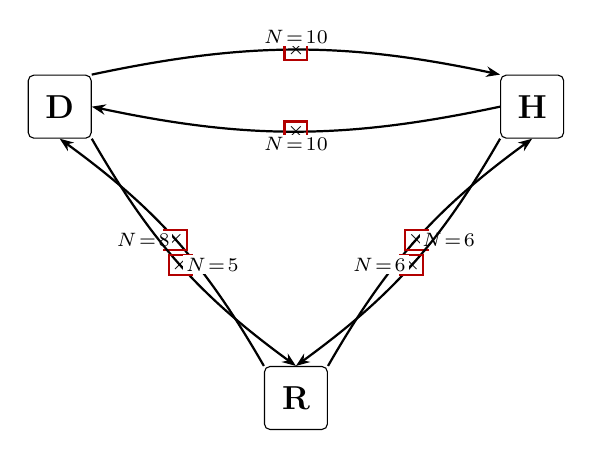
\begin{tikzpicture}[
    node distance=3.5cm,
    capability/.style={draw, rectangle, rounded corners=2pt, minimum size=8mm, font=\large\bfseries},
    arr/.style={-{Stealth[length=5pt]}, thick},
    cross/.style={draw=red!70!black, thick, inner sep=1pt, font=\scriptsize\bfseries},
    lbl/.style={font=\scriptsize, fill=white, inner sep=1pt},
  ]
  % Nodes in a triangle
  \node[capability] (S) at (0, -3.2) {R};
  \node[capability] (D) at (-3, 0.5) {D};
  \node[capability] (H) at (3, 0.5) {H};

  % S -> D (curved left)
  \draw[arr] (S.north west) to[bend right=12] coordinate[midway] (SD) (D.south);
  \node[cross] at (SD) {$\times$};
  \node[lbl, left=1pt of SD] {$N\!=\!8$};

  % D -> S (curved left)
  \draw[arr] (D.south east) to[bend right=12] coordinate[midway] (DS) (S.north);
  \node[cross] at (DS) {$\times$};
  \node[lbl, right=1pt of DS] {$N\!=\!5$};

  % S -> H (curved right)
  \draw[arr] (S.north east) to[bend left=12] coordinate[midway] (SH) (H.south);
  \node[cross] at (SH) {$\times$};
  \node[lbl, right=1pt of SH] {$N\!=\!6$};

  % H -> S (curved right)
  \draw[arr] (H.south west) to[bend left=12] coordinate[midway] (HS) (S.north);
  \node[cross] at (HS) {$\times$};
  \node[lbl, left=1pt of HS] {$N\!=\!6$};

  % D -> H (upper arc)
  \draw[arr] (D.north east) to[bend left=12] coordinate[midway] (DH) (H.north west);
  \node[cross] at (DH) {$\times$};
  \node[lbl, above=1pt of DH] {$N\!=\!10$};

  % H -> D (lower arc)
  \draw[arr] (H.west) to[bend left=12] coordinate[midway] (HD) (D.east);
  \node[cross] at (HD) {$\times$};
  \node[lbl, below=1pt of HD] {$N\!=\!10$};
\end{tikzpicture}
\caption{Full independence structure. All six pairwise non-implications are proved by Lean-verified finite counterexamples at the indicated sizes. No capability implies any other.}
\label{fig:independence}
\end{figure}

\begin{theorem}[Full Independence]
\label{thm:independence}
No capability implies any other. Specifically, all six pairwise non-implications hold:
\begin{enumerate}
  \item $R \not\Rightarrow D$: An extensional 2-pointed magma of size $8$ satisfying R contains a classifier element but fails the global dichotomy condition.
  \item $R \not\Rightarrow H$: An extensional 2-pointed magma of size $6$ satisfying R has 4 core elements (enough for $\ICP$ to be non-vacuous) but no triple satisfies the $\ICP$.
  \item $D \not\Rightarrow H$: An extensional 2-pointed magma of size $10$ satisfying both R and D has no triple satisfying the $\ICP$.
  \item $H \not\Rightarrow D$: An extensional 2-pointed magma of size $10$ satisfies $\ICP$ but violates the classifier dichotomy.
  \item $D \not\Rightarrow R$: An extensional 2-pointed magma of size $5$ satisfies the classifier dichotomy but admits no retraction pair.
  \item $H \not\Rightarrow R$: An extensional 2-pointed magma of size $6$ satisfies $\ICP$ but admits no retraction pair.
\end{enumerate}
\end{theorem}

\begin{proof}
Each direction is proved by exhibiting a concrete Cayley table and verifying the claimed properties by \texttt{native\_decide} (or \texttt{decide} for $N \leq 8$). The tables are:

\paragraph{$R \not\Rightarrow D$ ($N\!=\!8$, the Countermodel).}
An $8 \times 8$ Cayley table (Appendix~\ref{app:tables}) defining an $\FRM$ with $s = 2$, $r = 3$. The retraction pair works: $r \dotop (s \dotop x) = x$ for all core $x \in \{2,\ldots,7\}$ (e.g., $3 \dotop (2 \dotop 5) = 3 \dotop 6 = 5$). Element~4 is a classifier: its row on core is $(0,0,0,0,1,0) \subseteq \{z_1, z_2\}$. But element~5's row on core is $(6, 2, 1, 1, 1, 1)$ --- it maps core inputs 2 and 3 to non-absorber values (6 and 2), while mapping inputs 4--7 to absorber value~1. This mixed behavior violates the classifier dichotomy: element~5 is neither entirely absorber-valued nor entirely non-absorber-valued on core. Self-representation holds; self-description fails. Lean file: \texttt{Countermodel.lean}.

\paragraph{$R \not\Rightarrow H$ ($N\!=\!6$, structural).}
A $6 \times 6$ Cayley table (Appendix~\ref{app:tables}) defining an extensional 2-pointed magma with a retraction pair ($s = r = 2$, an involution on core) but no $\ICP$. The core has 4 elements --- more than the 3 pairwise distinct witnesses $\ICP$ requires --- yet no triple satisfies the $\ICP$. Lean proves $\neg\,\texttt{HasICP}$ by exhaustive search via \texttt{decide}. Lean file: \texttt{E2PM.lean}, theorem \texttt{s\_not\_implies\_icp\_structural}.

\paragraph{$D \not\Rightarrow H$ ($N\!=\!10$).}
A $10 \times 10$ Cayley table satisfying D (and also R). Lean proves that no triple $(a, b, c)$ of pairwise distinct non-absorbers satisfies the $\ICP$, by exhaustive search via \texttt{native\_decide}. Lean files: \texttt{Countermodels10.lean}, \texttt{ICP.lean} (theorem \texttt{dNotH\_no\_icp}).

\paragraph{$H \not\Rightarrow D$ ($N\!=\!10$).}
A $10 \times 10$ Cayley table defining an extensional 2-pointed magma with a retraction pair, satisfying $\ICP$ (witnessed by $a\!=\!8, b\!=\!6, c\!=\!7$), yet violating the dichotomy: element~5 has both absorber-valued and non-absorber-valued outputs on core. Lean file: \texttt{Countermodels10.lean}.

\paragraph{$D \not\Rightarrow R$ ($N\!=\!5$).}
A $5 \times 5$ Cayley table defining an extensional 2-pointed magma with the classifier dichotomy (classifier at index~2, non-classifiers at 3 and 4), but admitting no retraction pair. Lean proves $\neg\,\texttt{HasRetractPair}$ by exhaustive search over all candidate pairs via \texttt{decide}. Lean file: \texttt{E2PM.lean}, theorem \texttt{d\_not\_implies\_s}.

\paragraph{$H \not\Rightarrow R$ ($N\!=\!6$).}
A $6 \times 6$ Cayley table defining an extensional 2-pointed magma satisfying $\ICP$ (witnessed by $a\!=\!2, b\!=\!4, c\!=\!5$), but admitting no retraction pair. Lean file: \texttt{E2PM.lean}, theorem \texttt{h\_not\_implies\_s}.

All tables are generated by Z3 SAT solver and independently verified. The Cayley tables are frozen in the repository for reproducibility.
\end{proof}

\paragraph{Methodology.}
Each counterexample was found by encoding the relevant capability axioms (and the negation of the target capability) as a SAT problem over an $n \times n$ Cayley table, then solving with Z3. The search space is $n^{n^2}$ (all possible binary operations on $\Fin(n)$); the axioms reduce this to a manageable constraint system. The sizes $N\!=\!8$ and $N\!=\!10$ were discovered by incrementing $n$ from the minimum until SAT returned a model. Once found, each table was frozen in \texttt{counterexamples.json} and independently verified in Lean. The counterexample sizes are \emph{not} claimed to be universally minimal: they are minimal among the role assignments tested (SAT returned UNSAT at all smaller sizes with the same role assignments), but different role assignments or overlapping encodings could in principle yield smaller witnesses. We state no lower bounds on counterexample size.

\paragraph{Interpretation.}
The $H \not\Rightarrow D$ direction shows that an algebra can internalize a non-trivial composition pattern, as captured by the $\ICP$, without also satisfying the classifier dichotomy. Thus self-execution in our sense does not force the organizational separation expressed by D.

\paragraph{Decomposition of self-simulation.}
The independence result decomposes self-simulation into three independently satisfiable components. An algebra can encode and decode without classifying (R without D). An algebra can classify without encoding (D without R). An algebra can internally compose without classifying or encoding (H without R or D). Structured self-simulation uses all three simultaneously in the $N\!=\!5$ and $N\!=\!6$ witnesses (Theorems~\ref{thm:selfsim5} and~\ref{thm:selfsim6}), but the algebra can acquire each capability independently. Whether self-simulation \emph{strictly requires} all three depends on the precise formalization; what the independence result establishes is that no capability algebraically forces any other.

% ══════════════════════════════════════════════════════════════
\section{Coexistence}
\label{sec:bound}
% ══════════════════════════════════════════════════════════════

\begin{theorem}[No ICP at $N\!=\!4$]
\label{thm:no-icp-4}
No extensional 2-pointed magma of size $4$ satisfies the $\ICP$. The core $\{2,3\}$ has only 2 elements, but $\ICP$ requires 3 pairwise distinct non-absorbers. Lean: \texttt{Witness5.lean}, \texttt{no\_icp\_at\_4}.
\end{theorem}

\begin{theorem}[Coexistence Witness]
\label{thm:bound}
The three capabilities R, D, and H are simultaneously satisfiable. A Lean-verified witness exists at $N\!=\!5$, which is optimal by Theorem~\ref{thm:no-icp-4}.
\end{theorem}

\begin{proof}
A concrete $5 \times 5$ Cayley table is exhibited with $s\!=\!r\!=\!2$ (identity on core), classifiers $\tau \in \{3,4\}$, and $\ICP$ witnessed by $a\!=\!3, b\!=\!2, c\!=\!4$. The retraction pair collapses to a single element ($s\!=\!r$) which doubles as the $\ICP$'s core-preserving map; since $b$ is the identity, the factorization $a \cdot x = c \cdot (b \cdot x)$ reduces to $a \cdot x = c \cdot x$ on core --- two classifiers agreeing on core but distinguished by their absorber columns. The lower bound is pigeonhole: at $N\!=\!4$, the core $\{2,3\}$ has only 2 elements, but $\ICP$ requires 3 pairwise distinct non-absorbers (\texttt{no\_icp\_at\_4}). Lean file: \texttt{Witness5.lean}, theorem \texttt{sdh\_witness\_5}. A $6 \times 6$ witness with $s \neq r$ is also verified (\texttt{Witness6.lean}).
\end{proof}

\begin{proposition}[Separated-Role Witness]
\label{thm:separated}
There is a witness at $N\!=\!10$ in which the principal R+D+H roles (2 absorbers, 2 retraction pair, 1 classifier, 3 $\ICP$ witnesses) occupy 8 distinct elements, with 2 additional elements serving the enrichment axioms (Branch and Y, defined in Section~\ref{sec:icp}).
\end{proposition}

\begin{proof}
A concrete $10 \times 10$ Cayley table (Appendix~\ref{app:tables}) satisfies all three capabilities with 10 distinct role assignments. Additionally, the enrichments Branch and Y hold. Lean file: \texttt{Witness10.lean}.
\end{proof}

\paragraph{Minimum cardinality.}
$N\!=\!5$ is the optimal minimum for R+D+H coexistence (Lean-verified; \texttt{Witness5.lean}). The witness uses $s = r$ (identity on core), two classifiers, and one non-classifier: the retraction pair member doubles as the ICP's core-preserving element. At $N\!=\!4$ the core has only 2 elements but ICP requires 3 pairwise distinct non-absorbers, so $N\!=\!4$ is impossible (\texttt{no\_icp\_at\_4}).

The $N\!=\!5$ witness reveals how thin the three properties can become simultaneously. The retraction pair is the identity on core ($s = r$, no actual encoding work), and the ICP factorization $a \dotop x = c \dotop (b \dotop x)$ collapses to $a \dotop x = c \dotop x$ (row equality on core between two classifiers differing only on absorber columns). The three capabilities are formally present but barely interacting. The $N\!=\!6$ witness with $s \neq r$ (Theorem~\ref{thm:selfsim6}) is the more informative example: the retraction pair does genuine encoding, the ICP factorization is non-degenerate, and the roles do not trivially overlap. We retain the general definitions (allowing $s = r$) since the algebraic results --- independence, injectivity, no-associativity --- hold regardless.

% ══════════════════════════════════════════════════════════════
\section{Related Work}
\label{sec:related}
% ══════════════════════════════════════════════════════════════

\paragraph{Partial and total combinatory algebras.}
PCAs~\cite{vanoosten08,longley15} and TCAs~\cite{bethke88} provide the standard algebraic framework for realizability and computability. PCA theory has a rich structural theory: morphisms between PCAs, the lattice of PCA quotients, and totalizability~\cite{bethke96} all involve detailed analysis of the application operation. PCA theory does study which elements realize which functions. However, this analysis concerns representability and inter-PCA relationships, not the \emph{partition} of elements into behavioral types by their row structure --- whether classifiers and non-classifiers form disjoint classes, or what algebraic constraints (no associativity, no right identity) follow from that partition. Bethke and Klop~\cite{bethke96} proved that some PCAs cannot be extended to total ones, a structural result about the relationship between partiality and totality. The K-infinity theorem (our Theorem~\ref{thm:k-infinity}) shows that nontrivial S+K algebras must be infinite, explaining why finite algebras fall outside this framework and why our setting requires a different combinator basis.

\paragraph{Turing categories.}
Cockett and Hofstra~\cite{cockett08} define a Turing category as a cartesian restriction category with a Turing object~$A$ and a Turing morphism $\bullet : A \times A \to A$ that universally simulates all morphisms in the category. The Structure Theorem establishes that PCAs and Turing categories are two views of the same concept. Turing objects have cardinality ``one or infinite''~\cite{cockett08}, ruling out nontrivial finite Turing objects. The Turing morphism is described as ``the heart of the whole structure'' but its algebraic properties --- row structure, element classification, associativity constraints --- are not studied. Our self-simulation definition (Definition~\ref{def:selfsim}) resembles the Turing morphism's universality condition, but operates on the term algebra of a finite ground set and has algebraic consequences (Theorem~\ref{thm:injectivity}: injectivity of partial application) that Turing morphisms lack. Where Turing categories distribute computational roles across distinct objects (programs, data, evaluators), our finite algebras develop the same roles internally as emergent behavioral regions within a single carrier set: absorbers encode failure, classifiers provide absorber-valued judgment, and the retraction pair provides encoding.

\paragraph{Reflective towers.}
Smith's 3-Lisp~\cite{smith84} introduced the reflective tower --- an infinite chain of meta-interpreters. Subsequent work~\cite{friedman84,danvy88} explored reification, intensions, and live meta-modification in reflective towers. Amin and Rompf~\cite{amin18} showed how to compile through the tower via stage polymorphism. All of these systems combine self-representation, self-description, and self-execution without separating them. Our contribution is to show that in finite extensional 2-pointed magmas, the three capabilities are separable: no capability implies any other.

\paragraph{Self-interpretation.}
Mogensen~\cite{mogensen92} constructs self-interpreters for the $\lambda$-calculus. Brown and Palsberg~\cite{brown16} show that self-interpretation is possible in strongly-normalizing typed languages, contradicting earlier impossibility results. These works study self-interpretation (our R) but do not address the independence of R from D or H.

\paragraph{Independence in finite algebra.}
Independence and non-implication results between equational properties have a long history in universal algebra, from Birkhoff's characterization of equational classes~\cite{burris81} to Mal'cev conditions characterizing implications between properties of varieties. Our results operate at a different level: we separate \emph{operational} properties (retraction pairs, classifier partitions, factorizations in the left-regular representation) rather than equational identities, and our base class --- finite extensional 2-pointed magmas --- is not a variety in the Birkhoff sense (extensionality is a quasi-identity, not an equation). To our knowledge, the pairwise independence of retraction pairs, classifier dichotomies, and factorization properties in finite magmas has not been previously established. The SAT-find-then-Lean-verify methodology is related to the use of automated tools such as Mace4~\cite{mccune10} for counterexample search in algebra, though we use Z3 for constraint solving and Lean~4 for independent formal verification.

\paragraph{Finite model theory and machine-checked proofs.}
Independence results via finite counterexamples are standard in finite model theory~\cite{libkin04}. Each Cayley table is frozen in the Lean source and verified by the kernel, eliminating transcription errors. The sizes involved ($N\!=\!5$ through $N\!=\!10$) are small enough for \texttt{decide}/\texttt{native\_decide} but large enough that hand-verification of all conditions would be error-prone. The universal algebraic theorems (no-associativity, decomposition invariance, ICP equivalence) are proved by pure equational reasoning without \texttt{decide}, and hold for all finite sizes.

% ══════════════════════════════════════════════════════════════
\section{Discussion}
\label{sec:discussion}
% ══════════════════════════════════════════════════════════════

\paragraph{The classifier dichotomy is organizational.}
D organizes elements into coherent categories --- classifiers that test and non-classifiers that transform. The $H \not\Rightarrow D$ result shows that an algebra can internalize composition without this organization. D contributes semantic structure rather than compositional behavior.

\paragraph{Why magmas?}
Magmas are not a limitation but a necessity, for two independent reasons. First, the K-infinity theorem (Theorem~\ref{thm:k-infinity}) shows that nontrivial combinatory algebras with $\mathbf{s}$ and $\mathbf{k}$ must be infinite: the $\mathbf{k}$ combinator is a non-surjective injection on any finite set with $\geq 2$ elements. Finite self-description requires a different combinator basis --- one without a K-like projector --- and our extensional 2-pointed magmas provide exactly this. Second, Theorem~\ref{thm:no-assoc} shows that associativity forces any classifier to have a constant row, collapsing it to an absorber. Combined with the no-right-identity result (Theorem~\ref{thm:no-rid}), this independently rules out the entire classical algebraic hierarchy: no semigroup, monoid, group, or ring can support the classifier dichotomy alongside a retraction pair. Self-description lives outside both the PCA/TCA framework (by cardinality) and the classical algebraic hierarchy (by associativity). This connects to the broader observation that reflective systems are inherently non-associative: $\lambda$-calculus application is non-associative ($(f\,g)\,x \neq f\,(g\,x)$ in general). The no-associativity theorem shows this is algebraically forced, not a design accident.

\paragraph{The role of extensionality.}
Extensionality (distinct elements have distinct rows) is load-bearing throughout. Without it, the partial application injectivity theorem (Theorem~\ref{thm:injectivity}) fails: the final step derives $a_1 = a_2$ from identical rows, which requires extensionality. Without it, the no-associativity proof fails: Step~4 derives $\tau = v$ from identical rows. Without it, any constant-row element trivially satisfies both classifier and non-classifier conditions, making the three-category decomposition degenerate. Extensionality is not merely a convenience --- it is the condition that makes element-level classification meaningful. An element's identity \emph{is} its row in the Cayley table; extensionality formalizes this.

\paragraph{Why these three properties?}
The definitions of R, D, and H are motivated by two complementary considerations. First, each corresponds to a step in the self-simulation pipeline (Figure~\ref{fig:flow}): R provides encoding/decoding, D provides element classification, and H internalizes composition. A skeptical reader might ask why \emph{these} three steps rather than others; the answer is that R, D, and H are the independently formalizable algebraic properties that emerge when one asks what a self-simulation pipeline requires, and the independence theorem confirms they cannot be collapsed. Second, each property connects to a standard algebraic or categorical concept. Capability~R is a section-retraction pair~\cite{maclane71}: two core elements $s, r$ satisfying $r \circ s = \mathrm{id}$ on core. Capability~D parallels the partition of morphisms into characteristic and non-characteristic in presheaf categories~\cite{johnstone02}; the global dichotomy condition (no partial classifiers) is the finite-algebraic analogue of requiring a subobject classifier to be total. Capability~H asks for a non-trivial factorization in the left-regular representation $\{L_a\}$. The D and H connections are analogies, not formal correspondences: whether D is equivalent to a subobject-classifier condition or H to a standard categorical universal property remains open.

\paragraph{Why the independence holds.}
The independence of D and H reflects incompatible row constraints under finiteness. A classifier's row is fully committed to absorber values on core: every core input maps to $z_1$ or $z_2$. An ICP witness $a$ requires $a \dotop x = c \dotop (b \dotop x)$ with at least two distinct values on core --- its row must be non-trivially structured. These demands are incompatible for any single element, so different elements must carry these roles. The independence holds because finiteness limits the total supply of elements and constrains which row patterns can coexist under extensionality. The $H \not\Rightarrow D$ direction has the same character: an ICP triple $(a, b, c)$ constrains three rows to satisfy a factorization equation, but this imposes no absorber-output condition on any fourth element.

\paragraph{The infinite boundary.}
In infinite carriers where the set of left-multiplication maps is unconstrained --- such as the full function space over a countable set --- the row-scarcity constraint dissolves. The carrier is large enough to accommodate elements with arbitrary row patterns, and the tension between classifier rows and factorization rows need not arise. Whether the independence survives in specific infinite algebraic settings is open. This is an observation about resource limitations, not a theorem about Turing completeness: the precise conditions under which the independence transfers require defining the relevant algebraic properties for infinite carriers, which is beyond this paper's scope.

\paragraph{R as a separate design choice.}
The independence of R from D and H plausibly extends beyond finite magmas. A faithful internal encoding --- a section-retraction pair on the carrier --- is a separate design choice from classification or composition. Mogensen's self-interpreter for the $\lambda$-calculus~\cite{mogensen92} requires an explicit quoting convention; without it, the calculus is computationally universal but lacks internal self-representation. This suggests that the R independence is not an artifact of finiteness but reflects a genuine structural distinction between having computational capabilities and having a faithful encoding of one's own elements as data.

\paragraph{Scope and limitations.}
Whether the three-capability separation appears in other settings ($\lambda$-calculus, typed systems, infinite algebras) is the primary open question. Theorem~\ref{thm:no-assoc} constrains the target: any such translation must work without associativity or identity. A categorical characterization of H as a universal property (stronger than the analogy above) is also open. Two further directions connect to the frameworks discussed in Section~\ref{sec:related}: (1)~the \emph{extraction theorem} --- do the emergent behavioral roles (absorbers, classifiers, non-classifiers) formally yield a Turing category when used as objects, with role-respecting elements as morphisms? (2)~the \emph{realizability connection} --- does the classifier dichotomy, viewed as a property of an underlying PCA, predict specific logical principles in the associated realizability topos?

\paragraph{The cost of legibility.}
Additional organizational axioms push the minimum coexistence size to $N\!=\!12$ (SAT-verified) and produce interpretable role structure; these are explored in a companion paper.

\paragraph{Realization freedom.}
Each capability admits multiple axiom forms; the independence result holds for all variants.

% ══════════════════════════════════════════════════════════════
\section{Conclusion}
% ══════════════════════════════════════════════════════════════

We have proved that three natural properties of finite extensional 2-pointed magmas --- self-representation~(R), the classifier dichotomy~(D), and the Internal Composition Property~(H) --- are pairwise independent. Reflective systems in practice use all three; the independence result shows that in finite extensional 2-pointed magmas, this usage is not algebraically forced. The six non-implications are machine-checked in Lean~4. The optimal $N\!=\!5$ coexistence witness (Theorem~\ref{thm:bound}) self-simulates (\texttt{SelfSim5.lean}), and the partial application injectivity theorem (Theorem~\ref{thm:injectivity}) shows that self-simulation forces discrimination. Associativity is incompatible with the classifier structure (Theorem~\ref{thm:no-assoc}), ruling out semigroups, monoids, groups, and rings as settings for self-description. All results are formalized in Lean~4 (90 theorems across 13 files, zero \texttt{sorry}).

\paragraph{Open problems.}
\begin{enumerate}
  \item \emph{Cross-formalism universality}: Does the three-capability separation appear in the $\lambda$-calculus, typed settings, or infinite algebras? The no-associativity obstruction (Theorem~\ref{thm:no-assoc}) constrains the target setting.
  \item \emph{Categorical characterization of H}: Is the ICP equivalent to a standard universal property (e.g., existence of a partial internal hom)?
\end{enumerate}

\paragraph{Artifact.}
All Lean files, counterexample tables, SAT reproduction scripts, and the 16-element reflective tower artifact are available at \url{https://github.com/stefanopalmieri/Kamea}.

% ══════════════════════════════════════════════════════════════
% References
% ══════════════════════════════════════════════════════════════

\begin{thebibliography}{20}

\bibitem{smith84}
Brian Cantwell Smith.
\newblock Reflection and semantics in {Lisp}.
\newblock In \emph{POPL}, pages 23--35, 1984.

\bibitem{friedman84}
Daniel P. Friedman and Mitchell Wand.
\newblock Reification: Reflection without metaphysics.
\newblock In \emph{LFP}, pages 348--355, 1984.

\bibitem{danvy88}
Olivier Danvy and Karoline Malmkj{\ae}r.
\newblock Intensions and extensions in a reflective tower.
\newblock In \emph{LFP}, pages 28--39, 1988.

\bibitem{amin18}
Nada Amin and Tiark Rompf.
\newblock Collapsing towers of interpreters.
\newblock In \emph{POPL}, Article 52, pages 1--33, 2018.

\bibitem{mogensen92}
Torben Mogensen.
\newblock Efficient self-interpretation in lambda calculus.
\newblock \emph{Journal of Functional Programming}, 2(3):279--291, 1992.

\bibitem{brown16}
Matt Brown and Jens Palsberg.
\newblock Breaking through the normalization barrier: A self-interpreter for {F-omega}.
\newblock In \emph{POPL}, pages 5--17, 2016.

\bibitem{maclane71}
Saunders Mac~Lane.
\newblock \emph{Categories for the Working Mathematician}.
\newblock Springer, 1971.

\bibitem{johnstone02}
Peter~T. Johnstone.
\newblock \emph{Sketches of an Elephant: A Topos Theory Compendium}, vol.~1.
\newblock Oxford University Press, 2002.

\bibitem{libkin04}
Leonid Libkin.
\newblock \emph{Elements of Finite Model Theory}.
\newblock Springer, 2004.

\bibitem{burris81}
Stanley Burris and H.~P. Sankappanavar.
\newblock \emph{A Course in Universal Algebra}.
\newblock Springer, 1981.

\bibitem{mccune10}
William McCune.
\newblock \emph{Prover9 and Mace4}.
\newblock \url{https://www.cs.unm.edu/~mccune/prover9/}, 2005--2010.

\bibitem{moura21}
Leonardo de~Moura and Sebastian Ullrich.
\newblock The {Lean}~4 theorem prover and programming language.
\newblock In \emph{CADE}, pages 625--635, 2021.

\bibitem{vanoosten08}
Jaap van~Oosten.
\newblock \emph{Realizability: An Introduction to its Categorical Side}.
\newblock Studies in Logic and the Foundations of Mathematics~152, Elsevier, 2008.

\bibitem{longley15}
John Longley and Dag Normann.
\newblock \emph{Higher-Order Computability}.
\newblock Theory and Applications of Computability, Springer, 2015.

\bibitem{bethke88}
Ingemarie Bethke.
\newblock \emph{Notes on Partial Combinatory Algebras}.
\newblock PhD thesis, Universiteit van Amsterdam, 1988.

\bibitem{bethke96}
Ingemarie Bethke and Jan~Willem Klop.
\newblock Collapsing partial combinatory algebras.
\newblock In \emph{Higher-Order Algebra, Logic, and Term Rewriting (HOA 1995)}, LNCS~1074, pages 16--48, Springer, 1996. \textsc{doi}: 10.1007/3-540-61254-8\_18.

\bibitem{cockett08}
J.~Robin~B. Cockett and Pieter Hofstra.
\newblock Introduction to {T}uring categories.
\newblock \emph{Annals of Pure and Applied Logic}, 156(2--3):183--209, 2008. \textsc{doi}: 10.1016/j.apal.2008.04.005.

\end{thebibliography}

% ══════════════════════════════════════════════════════════════
\appendix
% ══════════════════════════════════════════════════════════════

\section{Cayley Tables}
\label{app:tables}

All tables are extracted from the Lean source files and verified by \texttt{lake build}. Element $i$'s row is row~$i$; entry $(i,j)$ is $i \dotop j$.

\paragraph{$N\!=\!4$: Minimal R+D witness ($s = r$).}
Roles: $0 = z_1$, $1 = z_2$, $2 = \tau$, $3 = s = r$. \quad Lean: \texttt{CatKripkeWallMinimal.lean}, \texttt{kripke4}.

\medskip
{\small
\begin{tabular}{c|cccc}
$\dotop$ & 0 & 1 & 2 & 3 \\\hline
0 & 0 & 0 & 0 & 0 \\
1 & 1 & 1 & 1 & 1 \\
2 & 0 & 1 & 0 & 1 \\
3 & 0 & 0 & 2 & 3 \\
\end{tabular}}

\paragraph{$N\!=\!5$: Minimal R+D witness ($s \neq r$).}
Roles: $0 = z_1$, $1 = z_2$, $2 = s$, $3 = r$, $4 = \tau$. \quad Lean: \texttt{CatKripkeWallMinimal.lean}, \texttt{kripke5}.

\medskip
{\small
\begin{tabular}{c|ccccc}
$\dotop$ & 0 & 1 & 2 & 3 & 4 \\\hline
0 & 0 & 0 & 0 & 0 & 0 \\
1 & 1 & 1 & 1 & 1 & 1 \\
2 & 1 & 0 & 3 & 4 & 2 \\
3 & 0 & 2 & 4 & 2 & 3 \\
4 & 0 & 1 & 1 & 0 & 0 \\
\end{tabular}}

\paragraph{$N\!=\!5$: R+D+H Optimal Coexistence ($s = r$, self-simulates).}
Roles: $0 = z_1$, $1 = z_2$, $2 = s = r$ (identity on core, ICP $b$), $3 = \tau$ (classifier, ICP $a$, self-sim term), $4 = \tau_2$ (classifier, ICP $c$). \quad Lean: \texttt{Witness5.lean}, \texttt{SelfSim5.lean}.

\medskip
{\small
\begin{tabular}{c|ccccc}
$\dotop$ & 0 & 1 & 2 & 3 & 4 \\\hline
0 & 0 & 0 & 0 & 0 & 0 \\
1 & 1 & 1 & 1 & 1 & 1 \\
2 & 0 & 2 & 2 & 3 & 4 \\
3 & 0 & 0 & 0 & 1 & 0 \\
4 & 0 & 1 & 0 & 1 & 0 \\
\end{tabular}}

\paragraph{$N\!=\!6$: R+D+H Coexistence (role overlap).}
Roles: $0 = z_1$, $1 = z_2$, $2 = s$ (also ICP $a$), $3 = r$ (also ICP $b$), $4 = \tau$, $5 =$ ICP $c$. \quad Lean: \texttt{Witness6.lean}.

\medskip
{\small
\begin{tabular}{c|cccccc}
$\dotop$ & 0 & 1 & 2 & 3 & 4 & 5 \\\hline
0 & 0 & 0 & 0 & 0 & 0 & 0 \\
1 & 1 & 1 & 1 & 1 & 1 & 1 \\
2 & 3 & 3 & 4 & 2 & 5 & 3 \\
3 & 0 & 1 & 3 & 5 & 2 & 4 \\
4 & 0 & 0 & 1 & 0 & 1 & 1 \\
5 & 2 & 2 & 5 & 4 & 3 & 2 \\
\end{tabular}}

\paragraph{$N\!=\!8$: $R \not\Rightarrow D$ Counterexample.}
Roles: $0 = z_1$, $1 = z_2$, $2 = s$, $3 = r$, $4 =$ classifier, $5, 7 =$ mixed (violate dichotomy). \quad Lean: \texttt{Countermodel.lean}.

\medskip
{\small
\begin{tabular}{c|cccccccc}
$\dotop$ & 0 & 1 & 2 & 3 & 4 & 5 & 6 & 7 \\\hline
0 & 0 & 0 & 0 & 0 & 0 & 0 & 0 & 0 \\
1 & 1 & 1 & 1 & 1 & 1 & 1 & 1 & 1 \\
2 & 3 & 3 & 7 & 3 & 4 & 6 & 5 & 2 \\
3 & 0 & 1 & 7 & 3 & 4 & 6 & 5 & 2 \\
4 & 0 & 0 & 0 & 0 & 0 & 0 & 1 & 0 \\
5 & 6 & 2 & 6 & 2 & 1 & 1 & 1 & 1 \\
6 & 0 & 0 & 5 & 2 & 2 & 2 & 2 & 2 \\
7 & 2 & 2 & 2 & 1 & 2 & 2 & 6 & 3 \\
\end{tabular}}

\paragraph{$N\!=\!6$: $R \not\Rightarrow H$ Counterexample (structural).}
Roles: $0 = z_1$, $1 = z_2$, $2 = s = r$ (involution on core). Retraction pair holds; no triple satisfies $\ICP$ despite 4 core elements. \quad Lean: \texttt{E2PM.lean} (\texttt{sNoH6\_e2pm}).

\medskip
{\small
\begin{tabular}{c|cccccc}
$\dotop$ & 0 & 1 & 2 & 3 & 4 & 5 \\\hline
0 & 0 & 0 & 0 & 0 & 0 & 0 \\
1 & 1 & 1 & 1 & 1 & 1 & 1 \\
2 & 0 & 3 & 3 & 2 & 5 & 4 \\
3 & 2 & 4 & 5 & 5 & 1 & 4 \\
4 & 5 & 3 & 0 & 0 & 3 & 2 \\
5 & 4 & 2 & 2 & 2 & 2 & 2 \\
\end{tabular}}

\paragraph{$N\!=\!10$: $D \not\Rightarrow H$ Counterexample.}
Roles: $0 = z_1$, $1 = z_2$, $2 = s$, $3 = r$, $4 = \tau$. No triple satisfies $\ICP$. \quad Lean: \texttt{Countermodels10.lean} (\texttt{dNotH}), \texttt{ICP.lean} (\texttt{dNotH\_no\_icp}).

\medskip
{\footnotesize
\begin{tabular}{c|cccccccccc}
$\dotop$ & 0 & 1 & 2 & 3 & 4 & 5 & 6 & 7 & 8 & 9 \\\hline
0 & 0 & 0 & 0 & 0 & 0 & 0 & 0 & 0 & 0 & 0 \\
1 & 1 & 1 & 1 & 1 & 1 & 1 & 1 & 1 & 1 & 1 \\
2 & 3 & 3 & 2 & 3 & 4 & 5 & 6 & 7 & 9 & 8 \\
3 & 0 & 1 & 2 & 3 & 4 & 5 & 6 & 7 & 9 & 8 \\
4 & 0 & 0 & 1 & 1 & 1 & 1 & 1 & 1 & 1 & 1 \\
5 & 1 & 0 & 0 & 0 & 0 & 0 & 0 & 0 & 0 & 0 \\
6 & 2 & 3 & 9 & 9 & 9 & 9 & 9 & 9 & 9 & 8 \\
7 & 3 & 2 & 9 & 9 & 9 & 9 & 9 & 9 & 9 & 8 \\
8 & 1 & 0 & 1 & 0 & 1 & 1 & 1 & 1 & 0 & 0 \\
9 & 0 & 1 & 0 & 1 & 0 & 1 & 1 & 0 & 1 & 1 \\
\end{tabular}}

\paragraph{$N\!=\!10$: $H \not\Rightarrow D$ Counterexample.}
Roles: $0 = z_1$, $1 = z_2$, $2 = s$, $3 = r$, $4 = \tau$. $\ICP$ holds ($a\!=\!8, b\!=\!6, c\!=\!7$). Element~5 violates dichotomy. \quad Lean: \texttt{Countermodels10.lean} (\texttt{hNotD}).

\medskip
{\footnotesize
\begin{tabular}{c|cccccccccc}
$\dotop$ & 0 & 1 & 2 & 3 & 4 & 5 & 6 & 7 & 8 & 9 \\\hline
0 & 0 & 0 & 0 & 0 & 0 & 0 & 0 & 0 & 0 & 0 \\
1 & 1 & 1 & 1 & 1 & 1 & 1 & 1 & 1 & 1 & 1 \\
2 & 3 & 1 & 3 & 4 & 9 & 6 & 8 & 5 & 7 & 2 \\
3 & 0 & 1 & 9 & 2 & 3 & 7 & 5 & 8 & 6 & 4 \\
4 & 0 & 0 & 1 & 1 & 1 & 1 & 1 & 1 & 0 & 0 \\
5 & 0 & 0 & 2 & 0 & 0 & 0 & 0 & 0 & 3 & 1 \\
6 & 2 & 2 & 2 & 8 & 3 & 9 & 4 & 7 & 9 & 7 \\
7 & 8 & 3 & 2 & 8 & 3 & 9 & 4 & 7 & 3 & 1 \\
8 & 9 & 2 & 2 & 3 & 8 & 1 & 3 & 7 & 1 & 7 \\
9 & 2 & 2 & 2 & 2 & 4 & 7 & 6 & 7 & 2 & 0 \\
\end{tabular}}

\paragraph{$N\!=\!5$: $D \not\Rightarrow R$ Counterexample.}
No retraction pair exists. Element~2 is a classifier: row on core is $(1,0,0) \subseteq \{z_1, z_2\}$. Elements~3 and 4 are non-classifiers: all core outputs $\geq 2$. Dichotomy holds; no pair of core elements forms a retraction pair. \quad Lean: \texttt{E2PM.lean} (\texttt{dNoS\_e2pm}).

\medskip
{\small
\begin{tabular}{c|ccccc}
$\dotop$ & 0 & 1 & 2 & 3 & 4 \\\hline
0 & 0 & 0 & 0 & 0 & 0 \\
1 & 1 & 1 & 1 & 1 & 1 \\
2 & 0 & 0 & 1 & 0 & 0 \\
3 & 4 & 2 & 4 & 2 & 4 \\
4 & 2 & 2 & 3 & 3 & 3 \\
\end{tabular}}

\paragraph{$N\!=\!6$: $H \not\Rightarrow R$ Counterexample.}
No retraction pair exists. $\ICP$ holds: $a\!=\!2, b\!=\!4, c\!=\!5$ with $b$ core-preserving and $2 \dotop x = 5 \dotop (4 \dotop x)$ on core. \quad Lean: \texttt{E2PM.lean} (\texttt{hNoS\_e2pm}).

\medskip
{\small
\begin{tabular}{c|cccccc}
$\dotop$ & 0 & 1 & 2 & 3 & 4 & 5 \\\hline
0 & 0 & 0 & 0 & 0 & 0 & 0 \\
1 & 1 & 1 & 1 & 1 & 1 & 1 \\
2 & 3 & 3 & 2 & 2 & 2 & 4 \\
3 & 0 & 2 & 2 & 2 & 4 & 0 \\
4 & 4 & 3 & 2 & 2 & 4 & 5 \\
5 & 0 & 0 & 2 & 2 & 2 & 4 \\
\end{tabular}}

\paragraph{$N\!=\!10$: R+D+H Coexistence Witness (all roles distinct).}
R+D+H roles: $0 = z_1$, $1 = z_2$, $2 = s$, $3 = r$, $4 = \tau$, $8 = \eta$ (ICP $a$), $6 = g$ (ICP $b$, core-preserving), $7 = \rho$ (ICP $c$). Enrichment roles (not used in this paper's theorems): $5 = f$, $7 = \rho$ (Branch dispatch), $9 = Y$ (fixed point). \quad Lean: \texttt{Witness10.lean}.

\medskip
{\footnotesize
\begin{tabular}{c|cccccccccc}
$\dotop$ & 0 & 1 & 2 & 3 & 4 & 5 & 6 & 7 & 8 & 9 \\\hline
0 & 0 & 0 & 0 & 0 & 0 & 0 & 0 & 0 & 0 & 0 \\
1 & 1 & 1 & 1 & 1 & 1 & 1 & 1 & 1 & 1 & 1 \\
2 & 3 & 3 & 4 & 3 & 7 & 5 & 9 & 6 & 8 & 2 \\
3 & 0 & 1 & 9 & 3 & 2 & 5 & 7 & 4 & 8 & 6 \\
4 & 0 & 0 & 1 & 1 & 1 & 0 & 0 & 0 & 1 & 1 \\
5 & 2 & 2 & 7 & 2 & 8 & 9 & 4 & 3 & 4 & 2 \\
6 & 0 & 0 & 6 & 4 & 8 & 7 & 3 & 3 & 4 & 9 \\
7 & 2 & 2 & 6 & 4 & 8 & 9 & 4 & 3 & 4 & 9 \\
8 & 2 & 2 & 4 & 8 & 4 & 3 & 4 & 4 & 8 & 9 \\
9 & 3 & 4 & 7 & 3 & 9 & 2 & 2 & 9 & 2 & 3 \\
\end{tabular}}

\section{Proof Inventory}
\label{app:inventory}

All Lean files compile with \texttt{lake build}, zero \texttt{sorry}. Proof styles: \emph{Algebraic} = pure equational reasoning (no \texttt{decide}); \emph{decide} = verified by kernel computation ($N \leq 8$); \emph{native\_decide} = verified by compiled native code ($N = 10$).

\medskip
{\small
\begin{tabular}{lrcl}
\textbf{File} & \textbf{Thms} & \textbf{Style} & \textbf{Content} \\
\hline
CatKripkeWallMinimal & 17 & Algebraic & Decomposition, bounds, wall \\
NoCommutativity      &  3 & Algebraic & Asymmetry \\
Functoriality        &  4 & Algebraic & Invariance under iso \\
SelfSimulation       &  5 & Algebraic & Partial app.\ injectivity \\
ICP                  & 20 & Alg.+decide & ICP $\Leftrightarrow$ Compose+Inert \\
Countermodel         &  5 & decide & $R \not\Rightarrow D$ ($N\!=\!8$) \\
Countermodels10      &  9 & native\_dec. & $D \not\Rightarrow H$, $H \not\Rightarrow D$ \\
E2PM                 & 10 & decide & $D \not\Rightarrow R$, $H \not\Rightarrow R$, $R \not\Rightarrow H$ \\
Witness10            &  6 & native\_dec. & R+D+H at $N\!=\!10$ \\
Witness5             &  3 & decide & R+D+H at $N\!=\!5$, no ICP at $N\!=\!4$ \\
Witness6             &  3 & decide & R+D+H at $N\!=\!6$ \\
SelfSim5             &  2 & native\_dec. & Self-simulation at $N\!=\!5$ \\
SelfSim6             &  3 & native\_dec. & Self-simulation at $N\!=\!6$ \\
\hline
\textbf{Total}       & \textbf{90} & & \\
\end{tabular}}

\end{document}
